% Choose one to switch betweeen slides and handout
\documentclass[]{beamer}
%\documentclass[handout]{beamer}

% Video Meta Data
\title{Bitcoin, Blockchain and Cryptoassets}
\subtitle{Bitcoin Primer}
\author{Prof. Dr. Fabian Schär}
\institute{University of Basel}

% Config File
% Packages
\usepackage[utf8]{inputenc}
\usepackage{hyperref}
\usepackage{gitinfo2}
\usepackage{tikz}
\usepackage{amsmath}
\usepackage{mathtools}
\usepackage{bibentry}
\usepackage{xcolor}
\usepackage{colortbl} % Add colour to LaTeX tables
\usepackage{caption}
\usepackage[export]{adjustbox}
\usepackage{pgfplots} \pgfplotsset{compat = 1.17}
\usepackage{makecell}
\usepackage{fancybox}
\usepackage{ragged2e}
\usepackage{fontawesome}
\usepackage{seqsplit}
\usepackage{tabularx}

% Color Options
\definecolor{highlight}{rgb}{0.65,0.84,0.82}
\definecolor{focus}{rgb}{0.72, 0, 0}
\definecolor{lightred}{rgb}{0.8,0.5,0.5}
\definecolor{midgray}{RGB}{190,195,200}

% Beamer Template Options
\beamertemplatenavigationsymbolsempty
\setbeamertemplate{footline}[frame number]
\setbeamercolor{structure}{fg=black}
\setbeamercolor{footline}{fg=black}
\setbeamercolor{title}{fg=black}
\setbeamercolor{frametitle}{fg=black}
\setbeamercolor{item}{fg=black}
\setbeamercolor{}{fg=black}
\setbeamercolor{bibliography item}{fg=black}
\setbeamercolor*{bibliography entry title}{fg=black}
\setbeamercolor{alerted text}{fg=focus}
\setbeamertemplate{items}[square]
\setbeamertemplate{enumerate items}[default]
\captionsetup[figure]{labelfont={color=black},font={color=black}}
\captionsetup[table]{labelfont={color=black},font={color=black}}

\setbeamertemplate{bibliography item}{\insertbiblabel}

% Link Icon Command
\newcommand{\link}{%
    \tikz[x=1.2ex, y=1.2ex, baseline=-0.05ex]{%
        \begin{scope}[x=1ex, y=1ex]
            \clip (-0.1,-0.1)
                --++ (-0, 1.2)
                --++ (0.6, 0)
                --++ (0, -0.6)
                --++ (0.6, 0)
                --++ (0, -1);
            \path[draw,
                line width = 0.5,
                rounded corners=0.5]
                (0,0) rectangle (1,1);
        \end{scope}
        \path[draw, line width = 0.5] (0.5, 0.5)
            -- (1, 1);
        \path[draw, line width = 0.5] (0.6, 1)
            -- (1, 1) -- (1, 0.6);
        }
    }

% Read Git Data from Github Actions Workflow
% Defaults to gitinfo2 for local builds
\IfFileExists{gitInfo.txt}
	{\input{gitInfo.txt}}
	{
		\newcommand{\gitRelease}{(Local Release)}
		\newcommand{\gitSHA}{\gitHash}
		\newcommand{\gitDate}{\gitAuthorIsoDate}
	}

% Custom Titlepage
\defbeamertemplate*{title page}{customized}[1][]
{
  \vspace{-0cm}\hfill\includegraphics[width=2.5cm]{../config/logo_cif}
  \includegraphics[width=1.9cm]{../config/seal_wwz}
  \\ \vspace{2em}
  \usebeamerfont{title}\textbf{\inserttitle}\par
  \usebeamerfont{title}\usebeamercolor[fg]{title}\insertsubtitle\par  \vspace{1.5em}
  \small\usebeamerfont{author}\insertauthor\par
  \usebeamerfont{author}\insertinstitute\par \vspace{2em}
  \usebeamercolor[fg]{titlegraphic}\inserttitlegraphic
    \tiny \noindent \texttt{Release Ver.: \gitRelease}\\ 
    \texttt{Version Hash: \gitSHA}\\
    \texttt{Version Date: \gitDate}\\ \vspace{1em}
    
    
    \iffalse
  \link \href{https://github.com/cifunibas/Bitcoin-Blockchain-Cryptoassets/blob/main/slides/intro.pdf}
  {Get most recent version}\\
  \link \href{https://github.com/cifunibas/Bitcoin-Blockchain-Cryptoassets/blob/main/slides/intro.pdf}
  {Watch video lecture}\\ 
  
  \fi
  
  \vspace{1em}
  License: \texttt{Creative Commons Attribution-NonCommercial-ShareAlike 4.0 International}\\\vspace{2em}
  \includegraphics[width = 1.2cm]{../config/license}
}


% tikzlibraries
\usetikzlibrary{decorations.pathreplacing}
\usetikzlibrary{decorations.markings}
\usetikzlibrary{positioning}
\usetikzlibrary{calc}
\captionsetup{font=footnotesize}

%%%%%%%%%%%%%%%%%%%%%%%%%%%%%%%%%%%%%%%%%%%%%%
%%%%%%%%%%%%%%%%%%%%%%%%%%%%%%%%%%%%%%%%%%%%%%
\begin{document}


%%
\thispagestyle{empty}
\begin{frame}[noframenumbering]
	\titlepage
\end{frame}
%%%


%%%
\begin{frame}{Review}

What we already know: \\ 
\vspace{1em}
	\begin{enumerate}
		\item<1->{transactions = messages distributed over the bitcoin network}
		\item<2->{basis for adjustment of the ledger}
		\item<3->{only possibility to transfer funds}
		\item<4->{no accounts}
		\item<5->{all transactions are publicly viewable}
	\end{enumerate}
\end{frame}
%%%


%%%
\begin{frame}{How to transfer a bitcoin unit} %mehr dazu auf Bitcoin Wiki nicht gefunden

\begin{enumerate}
		\item<1->{create transaction message}
		\item<2->{cryptographically sign message}
		\item<3->{propagate transaction to other network participants}
		\item<4->{nodes check if transaction is valid and forward it to their connected nodes}
	\end{enumerate}	
\end{frame}
%%%


%%%
\begin{frame}{Content of a transaction} %Structure of a transaction
 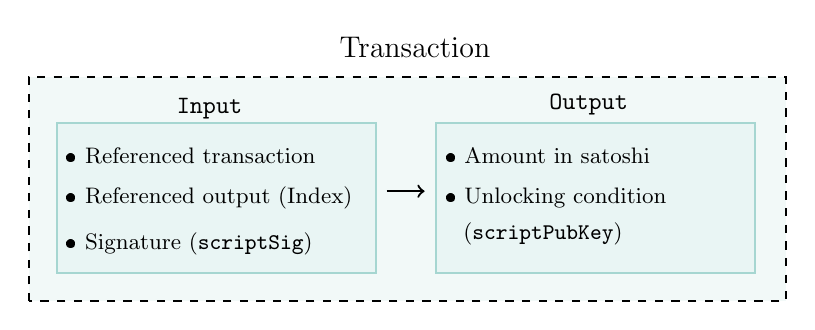
\begin{tikzpicture}[scale=0.9, every node/.style={scale=0.9}]
    
        \filldraw[yshift=-0.05cm, xshift=0.1cm,color = highlight!15, thick, draw=black, dashed] (-4,-4) rectangle ++(304pt,90pt) ;
    
        \filldraw[yshift=-0.05cm, xshift=0.1cm,color = highlight!25, thick, draw=highlight] (-3.6,-3.6) rectangle ++(128pt,60pt) ;
    
    \draw[->,thick] (1.15,-2.5) -- (1.685,-2.5) ;
    
    \draw[color=black] plot (-1.35,-1.6)   node[above] {\texttt{Input}};
    \draw[color=black] plot (-3.5,-2)   node[right] {\small{\textbullet{} {Referenced transaction}}};
    \draw[color=black] plot (-3.5,-2.6)   node[right] {\small{\textbullet{} Referenced output (Index)}};
    \draw[color=black] plot (-3.5,-3.25)   node[right] {\small{\textbullet{} Signature (\texttt{scriptSig})}};
    \draw[color=black] plot (1.55,-0.2) node [below]
    {\large{{Transaction}}};
    
    
        \filldraw[yshift=-0.05cm, xshift=0.1cm,color = highlight!25, thick, draw=highlight] (1.75,-3.6) rectangle ++(128pt,60pt) ;
    
    \draw[color=black] plot (4,-1.55)   node[above] {\texttt{Output}};
    \draw[color=black] plot (1.85,-2)   node[right] {\small{\textbullet{} Amount in satoshi}};
    \draw[color=black] plot (1.85,-2.6)   node[right] {\small{\textbullet{} Unlocking condition}};
    \draw[color=black] plot (2,-3.1)   node[right] {\small{ (\texttt{scriptPubKey})}};
    %\draw[color=black] plot (1.95,-3.2)   node[right] {\small{\textbullet{} Signatur / Lösung}};
    
    \end{tikzpicture}

\vspace{1em}
\begin{itemize}
  \item<2->{must contain at least one input and one output}
  \item<3->{sum of inputs must be at least as high as sum of outputs}
	\item<4->{credit can be divided to any number of output}
\end{itemize}
\end{frame}	
%%%


%%%
\begin{frame}{script condition}
\begin{itemize}
    \item<1->{transaction outputs contain condition}
    \item<2->{flexibility about what condition is defined}
    \item<3->{for example: condition can be met by signature with corresponding private key}
\end{itemize}
\end{frame}        
%%%


%%%
\begin{frame}{Unspent transaction outputs}
\begin{itemize}
    \item<1->{output can only be used once as input}
    \item<2->{unspent transaction output = UTXO}
    \item<3->{UTXO's are the systems value storage}
    \item<4->{stored on the blockchain and RAM of every full-node}
    \item<5->{bitcoin units can only exist in this form}
\end{itemize}    
\end{frame}
%%%


%%%
\begin{frame}{Example: transaction hierarchy}
\resizebox{10.7cm}{7cm}{
\input{../assets/figures/transaction-process.tex}
}
\end{frame}
%%%


%%%
\begin{frame}{transaction types}
\begin{columns}

\column{0.5\textwidth}
\vspace{1cm}
\input{../assets/figures/forwarding-transaction-type.tex} 
\vspace{0.4cm}
\input{../assets/figures/dividing-transaction-type.tex}

\column{0.5\textwidth}
\input{../assets/figures/aggregating-transaction-type.tex}
\vspace{0.5cm}
\input{../assets/figures/m-to-n-transaction-type.tex}

\end{columns}
\end{frame}
%%%


%%%
\begin{frame}{Input $\neq$ Output ?}
\begin{itemize}
    \item<1->{if value output $>$ value input $\rightarrow$ transaction invalid}
    \item<2->{if value output $<$ value input $\rightarrow$ miner gets difference}
    \end{itemize} 
    \vspace{2em}
\begin{center}
\uncover<3->{Setting a higher fee usually results in a faster inclution in a block.}
\end{center}  
\end{frame}
%%%


%%%
\begin{frame}{Schlussfolie}

\end{frame}
%%%

\end{document}
